% ===== 原文 pp.14–19（PDF p.24–29） =====
% [原文 p.14]
为了扭转 $\cN=4$，必须先 Wick 旋转到欧氏号差。因此我们将假定 $M$ 是黎曼四维流形，并假定我们所写下的作用量 $S$ 在路径积分中被理解为如下形式的权重因子
\[ \ee^{-S} \]
Wick 旋转后的欧氏群为 $Spin(4)\simeq SU(2)_l\times SU(2)_r$，相对于它，$Q$ 们作为 $(\mathbf{2},\mathbf{1})$ 变换，而 $\bar Q$ 们作为 $(\mathbf{1},\mathbf{2})$ 变换。

扭转是一个分两步的手续。从一个物理的\footnote{我们取“物理的”意指：满足 $\R^4$ 上相对论量子场论的通常性质，其中包括：酉性；欧氏不变性；具有常规动能项的正定作用量；无反常。}超对称场论（在我们的情形是 $\cN=4$ 超 YM）出发，第一步是通过对物质场自旋的巧妙重新定义来改造这个理论。具体地说，把欧氏转动群 $Spin(4)$ 经由一个同态 $\aleph:Spin(4)\to Spin(6)_R$ 嵌入 R-对称群 $Spin(6)_R$，并宣布扭转后的转动群 $Spin'(4)$ 由旧的 $Spin(4)$ 与其在 $Spin(6)_R$ 中的嵌入像的同时转动构成，即
\[ Spin'(4) \equiv (1\times\aleph)(Spin(4)) \subset Spin(4)\times Spin(6)_R \]

在扭转后的转动群下，$Q^i_{\dot A}$ 上的 R-对称指标 $i$ 相对于嵌入 $\aleph(Spin(4))\subset Spin(6)_R$ 分解为 $Spin(4)$ 的某个表示 $\mathbf{r}$；于是 $Q$ 们作为 $Spin'(4)$ 的 $(\mathbf{2},\mathbf{1})\otimes\mathbf{r}$ 变换。类似地，$\bar Q$ 们作为 $(\mathbf{1},\mathbf{2})\otimes\mathbf{l}$ 变换，其中 $\mathbf{l}$ 是 $Spin(4)$ 的某个表示。关键在于，嵌入 $\aleph$ 的选取使得 $(\mathbf{2},\mathbf{1})\otimes\mathbf{r}$ 或 $(\mathbf{1},\mathbf{2})\otimes\mathbf{l}$ 两者之一中含有一个单态，也就是说某个费米型对称性 $Q$ 在扭转后的转动群下作为标量变换。一个标量 $Q$ 在各坐标卡之间平凡地变换，因此这样的 $Q$ 在把时空取为一般弯曲流形 $M$ 之后仍将是理论的一个对称性。如此重新定义了场的自旋之后，扭转后的理论相当病态，因为它违反自旋-统计（特别地，它将不再是酉的）；这种酉性的缺失并不构成问题，只要我们谨慎地限制向该理论提出的问题以及它的用途。

% [Tutor Note: p.14 术语与记号。$\aleph$ 是原文用来记扭转同态 $Spin(4)\to Spin(6)_R$ 的符号（字形像希伯来字母 aleph），与基数 $\aleph_0$ 无关；“twisted rotation group”译作“扭转后的转动群”。可验证的判据：$\mathbf{2}\otimes\mathbf{2}=\mathbf{1}\oplus\mathbf{3}$（Clebsch–Gordan），故只有当 $\mathbf{r}$（或 $\mathbf{l}$）含 $SU(2)$ 的 $\mathbf{2}$ 时 $(\mathbf{2},\mathbf{1})\otimes\mathbf{r}$（或 $(\mathbf{1},\mathbf{2})\otimes\mathbf{l}$）才含单态——这正是 §2.4.1 中三种扭转的判定依据。]

扭转手法的第二步，是从这些单态中恰好挑出一个 $Q$（它必然在运动方程的意义上幂零），并把理论重新解释为：只关注被 $Q$ 湮灭的态与算子，模去 $Q$-正合的态与算子。这与规范理论的 BRST 荷完全类似，因此我们把这个 $Q$ 称为扭转后理论的 BRST 荷。我们将把对应于荷 $Q$ 的场变分记作 $\delta_Q$，并形式上宣布它具有奇统计。

扭转后的作用量取如下形式
\[ S = \delta_Q\int_M V + S_{top} \]
% [原文 p.15]
其中 $V$ 称为规范费米子（gauge fermion），而 $S_{top}$ 是仅依赖于理论场空间的连通分支的项，例如瞬子项 (2.2)。我们在本文中会一再遇到这种形式的作用量。它保证能动量张量是 $Q$-正合的，而这又保证 BRST 不变的场函数的关联函数与度规无关。的确，考虑如下形式的关联函数
\[ \langle\cO_1\ldots\cO_p\rangle = \int[D\Phi]\,\cO_1\ldots\cO_p\,\ee^{-S[\Phi]} \]
其中 $\Phi$ 是理论的场，而每个算子 $\cO_i$ 都被 $\delta_Q$ 湮灭（我们称这样的算子为理论的可观测量）。对 $M$ 上度规的任意形变 $\delta g^{\mu\nu}$ 计算变分，我们得到
\begin{align*}
\frac{\delta}{\delta g^{\mu\nu}}\int[D\Phi]\,\cO_1\ldots\cO_p\,\ee^{-S[\Phi]}
&= -\int[D\Phi]\,\cO_1\ldots\cO_p\,T_{\mu\nu}\,\ee^{-S[\Phi]} \\
&= -\int[D\Phi]\,\cO_1\ldots\cO_p\,\delta_Q\cV_{\mu\nu}\,\ee^{-S[\Phi]} \\
&= -\int[D\Phi]\,\delta_Q\Big\{\cO_1\ldots\cO_p\,\cV_{\mu\nu}\,\ee^{-S[\Phi]}\Big\} \\
&= 0
\end{align*}
这里我们用了能动量张量的定义 $T_{\mu\nu}=\delta S/\delta g^{\mu\nu}$、作用量的 BRST 不变性，并假定了可观测量与路径积分测度都与度规无关。这一类理论——在取 $Q$-上同调之后关联函数与度规无关——称为上同调拓扑场论。\footnote{严格说来，关联函数仍可能依赖度规的光滑结构；它们只是在度规的光滑形变下不变。}

% [Tutor Note: p.15 补出省略论证。最后一步“$=0$”用了两件事：其一，$\delta_Q\{\ldots\}$ 是全变分，而在路径积分中全变分积分为零（假定测度在 $\delta_Q$ 下不变、且没有边界）；其二，$e^{-S}$ 中 $S=\delta_Q\int V+S_{top}$ 的 $\delta_Q V$ 部分给出 $T_{\mu\nu}=\delta_Q\cV_{\mu\nu}$，而 $S_{top}$ 与度规无关。注意原文这里写的是对 $g^{\mu\nu}$（上指标）求变分，而 $T_{\mu\nu}=\delta S/\delta g^{\mu\nu}$ 给出的是混合位置的量；若改用 $\delta g_{\mu\nu}$ 变分，则 $T$ 的指标位置需相应调整，这不影响结论。]

应当强调，在平坦 $\R^4$ 上，扭转只不过是重新排列场的标号，因此扭转后的理论只是描述了原本物理理论的一个子扇区。

\subsection{\texorpdfstring{$\cN=4$ 的扭转}{N=4 的扭转}}

那么，把 $\cN=4$ 扭成 TFT 的方式有哪些？这就是所有同态 $\aleph:Spin(4)\to Spin(6)_R$ 的等价类，而后者又可以通过 $Spin(6)_R$ 的 $\mathbf{4}$ 在 $Spin(4)\simeq SU(2)_l\times SU(2)_r$ 嵌入下如何分解来刻画。最早在 [13] 中给出的答案是：共有三种可能的扭转理论：

% [Tutor Note: p.15 补出省略论证。“等价类”指同态相差 $Spin(6)_R$ 中的共轭（以及 $Spin(4)$ 中的自同构）。分类可归结为 $\mathbf{4}$ 在 $SU(2)_l\times SU(2)_r$ 下的分解方式：把 $\mathbf{4}$ 写成 $(\mathbf{2},\mathbf{1})\otimes\mathbf{r}$ 或 $(\mathbf{1},\mathbf{2})\otimes\mathbf{l}$，要求存在单态，等价于 $\mathbf{r}$ 或 $\mathbf{l}$ 含 $\mathbf{2}$；满足者恰有三种（DW、VW、GL），见下。]

\begin{itemize}
\item \emph{Donaldson-Witten（DW）扭转。} 使得 $\mathbf{4}\to(\mathbf{2},\mathbf{1})\otimes(\mathbf{1},\mathbf{1})\otimes(\mathbf{1},\mathbf{1})$ 的那种 $\aleph$ 选择给出一个带单个标量超荷的扭转理论。它对应于把 $\cN=4$ 视为带物质的 $\cN=2$、并用 $\cN=2$ 的 Donaldson-Witten 扭转 [45] 来扭转。本文不研究 Donaldson-Witten 扭转理论。

% [Tutor Note: p.15 原文笔误。DW 一行的分解 $\mathbf{4}\to(\mathbf{2},\mathbf{1})\otimes(\mathbf{1},\mathbf{1})\otimes(\mathbf{1},\mathbf{1})$ 维数不对：右端维数为 $2\times1\times1=2$，而左端是 $4$ 维。按相邻两行（VW 为 $\mathbf{2}\times\mathbf{2}=4$，GL 为 $\mathbf{2}\times\mathbf{2}=4$）的写法以及“DW 扭转只有一个标量超荷”这一事实，正确形式应为 $\mathbf{4}\to(\mathbf{2},\mathbf{1})\oplus(\mathbf{1},\mathbf{1})\oplus(\mathbf{1},\mathbf{1})$（$2+1+1=4$）；正是其中的两个单态说明存在标量超荷。]
% [原文 p.16]
\item \emph{Vafa-Witten（VW）扭转。} 使得 $\mathbf{4}\to(\mathbf{2},\mathbf{1})\otimes(\mathbf{2},\mathbf{1})$ 的嵌入给出一个带两个超荷的扭转理论。这两个超荷的所有线性组合作为 BRST 荷 $Q$ 的选择本质上是等价的。这一扭转理论在 [3] 中被用来检验 S-对偶的强耦合预言。

\item \emph{几何朗兰兹（GL）扭转。} 使得 $\mathbf{4}\to(\mathbf{2},\mathbf{1})\otimes(\mathbf{1},\mathbf{2})$ 的嵌入给出一个带两个标量超荷 $Q_l$ 与 $Q_r$ 的扭转理论；与 Vafa-Witten 理论相反，这两个标量超荷的不同线性组合并不等价。因此 GL-扭转实际上对应于由参数 $t$ 标记的一族 TFT。该扭转理论在 [1] 中被证明为从规范场论视角研究几何朗兰兹纲领提供了自然的框架，因此我们称它为 GL 扭转。
\end{itemize}

在随后的章节中，我们将研究 VW-与 GL-扭转理论（在扭转参数 $t$ 的某些取值处）的性质。Vafa-Witten 扭转理论的显式作用量与变分我们推迟到第 3 章再写，在那里将证明它自然地落在更广的一族 4d TFT 之内。现在让我们更详细地讨论 GL-扭转理论。

\section{GL-扭转理论}

\subsection{\texorpdfstring{$t$ 参数}{t 参数}}

首先考虑 BRST 荷的选择。如上所述，有两个（相互反对易的）标量超荷 $Q_l$ 与 $Q_r$，分别对应变分 $\delta_l$ 与 $\delta_r$，因此 $\delta_Q$ 可以是任意非零线性组合
\[ \delta_Q = u\,\delta_l + v\,\delta_r , \]
其中 $u,v\in\C$ 为两个参数。把 $\delta_Q$ 乘上整体复常数不改变理论的性质，因此 $(u,v)$ 应被视为互不等价选择的 $\C P^1$ 的齐次坐标。换一种方式，我们用
\[ t \equiv v/u , \qquad t\in\C\cup\{\infty\} \]
来参数化这一族互不等价的选择。

% [Tutor Note: p.16 补出省略论证。$\delta_Q^2=0$ 对任意 $(u,v)$ 成立，因为 $\delta_l^2=\delta_r^2=0$ 且 $\{\delta_l,\delta_r\}=0$（原文称之为“相互反对易”）；这正是 $(u,v)\in\C^2\setminus\{0\}$ 的模空间是 $\C P^1$ 的前提。核对：若两个标量超荷的线性组合不等价，则参数族应为一维复流形；GL-扭转的 $\C P^1$ 恰与之一致，而 VW 扭转的“所有线性组合等价”把 $\C P^1$ 塌缩成一点、因而不出现扭转参数。]

在 $t$ 处的 GL-扭转理论与在 $-t$ 处的理论通过 GL-扭转作用量的 R-对称群 $SU(4)_R$ 的中心的作用而平凡地相联系 [1]；不过，模去 $t\to-t$，$t$ 的其他所有选择都给出性质互不相同的 TFT。\footnote{如 [1] 中所讨论的，当四维流形 $M$ 具有定向反转对称性时，理论具有一个反转瞬子数符号的对称性；这导致 $t$ 处的理论与 $1/t$ 处的理论之间多出一个对称性。} 我们上面说过，左手超荷
% [原文 p.17]
在 S-对偶下被乘上一个相位，而右手超荷被乘上相反的相位。由此我们可以推断 S-对偶对 $t$ 参数的作用为
\[ t \longrightarrow \frac{\tau}{\abs{\tau}}\,t \]

% [Tutor Note: p.16–17 可验证的自洽检验。$t\to-t$ 的等价性可以独立核对：由 (2.3) 之后的式子，$\Psi=\frac{\theta}{2\pi}+\frac{4\pi\ii}{e^2}\frac{t^2-1}{t^2+1}$ 只依赖 $t^2$，故 $t\to-t$ 不改变 $\Psi$，而原文又说 GL-扭转理论的种种性质只通过 $\Psi$ 依赖 $t,e^2,\theta$——这印证了 $t$ 与 $-t$ 的等价。同样地，$t\to1/t$ 只在 $M$ 有定向反转对称性时才成为对称性（见脚注），这与 $\Psi$ 在 $t\to1/t$ 下变为 $\frac{\theta}{2\pi}-\frac{4\pi\ii}{e^2}\frac{t^2-1}{t^2+1}$（即 $\theta$ 与瞬子项的符号同时反号）一致。]

当 $\theta=0$ 时，可以把 S-对偶的作用想象为 $t$ 取值的黎曼球面上的一个 $\pi/2$ 旋转：

\begin{figure}[htbp]
\centering
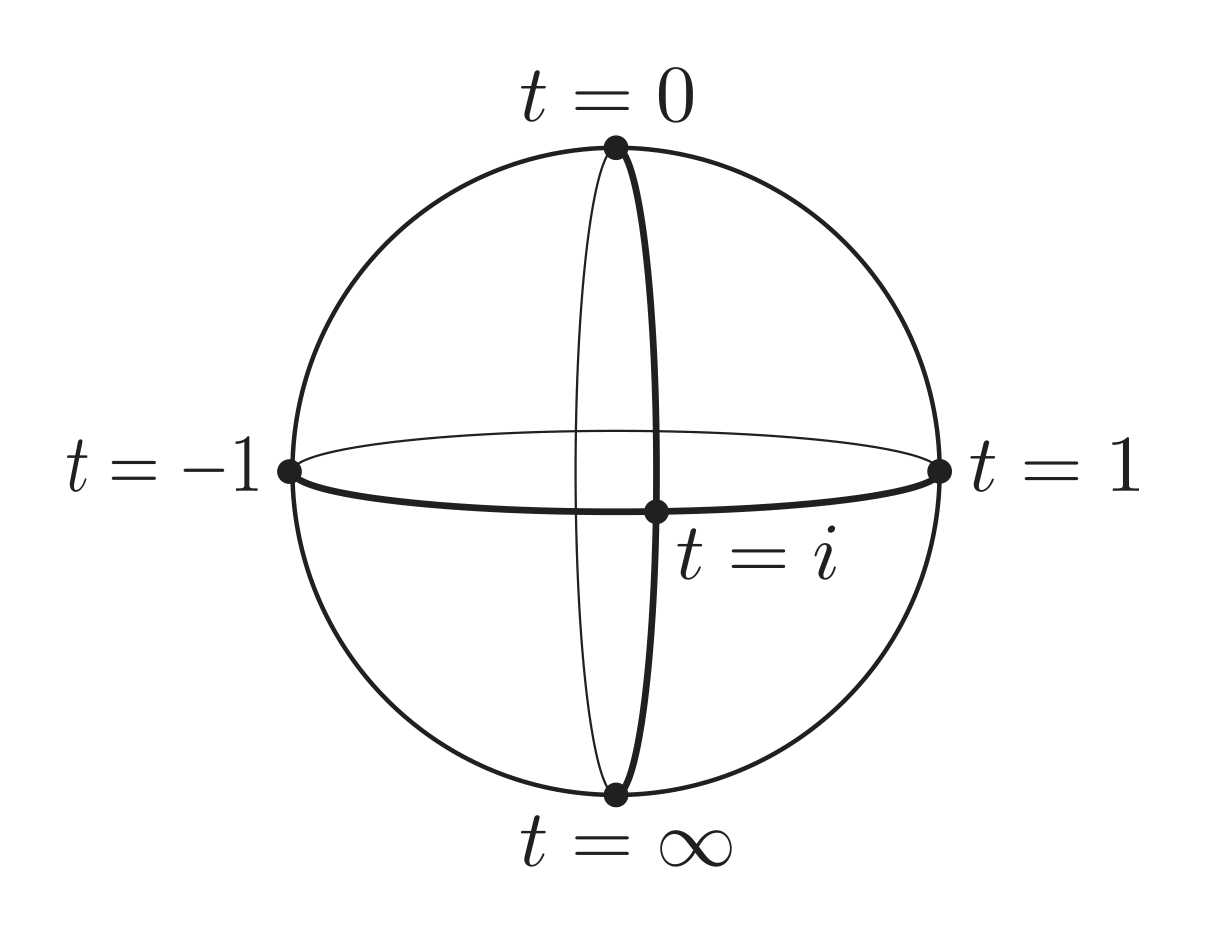
\includegraphics[width=0.5\textwidth]{fig21.png}
\figtitle{2.1}{扭转参数 $t$ 取值于 $\C\cup\{\infty\}$。}
\end{figure}

% [Tutor Note: p.17 图 2.1 与 $t$ 的旋转核对。图中 $t=0$ 在北极、$t=\infty$ 在南极，赤道即 $\abs{t}=1$，其上标出 $t=1$（右）、$t=-1$（左）、$t=\ii$（前方中点），未标 $t=-\ii$。核对 $\pi/2$ 旋转：$\theta=0$ 时 $\tau/|\tau|=\ii$，故 $t\mapsto\ii t$，它把 $1\to\ii\to-1\to-\ii\to1$ 循环——这正是图中赤道上四点被轮换的方式，也说明为什么只标出 $\pm1$ 与 $\ii$ 就足以刻画这个旋转。]

我们特别关心 GL-扭转理论在三个取值处的性质：$t=\ii$、$t=1$ 与 $t=0$；谈到这三个理论时，我们把“$t=\ii$”理解为“扭转参数为 $t=\ii$ 的 GL-扭转 TFT”的简写。$t=\ii$ 与 $t=1$ 两个理论由对偶互换，而在 [1] 中这两个 TFT 之间的对偶被证明为研究几何朗兰兹纲领提供了自然的框架。另一方面，$t=0$ 的理论是自对偶的，而在 [35] 中它被证明为研究量子几何朗兰兹（几何朗兰兹的一个涉及量子参数的推广）提供了自然的框架。

\subsection{GL-扭转理论的场含量、作用量与变分}

现在我们详细考察 GL-扭转理论在扭转参数 $t\in\C\cup\{\infty\}$ 的各种取值处的场含量、BRST 变分与作用量。

设 $P$ 是四维流形 $M$ 上的主 $G$-丛。按照 GL 扭转改造 $\cN=4$ 各场的自旋之后，玻色场由一个规范场 $A$（$P$ 上的联络）以及下列取值于丛 $ad\,P$ 的形式组成：
\begin{gather*}
\sigma \in \Omega^0(M, ad\,P)\otimes\C \\
\phi \in \Omega^1(M, ad\,P)
\end{gather*}
其中 $\sigma$ 是一个复 0-形式，由 $ad\,P$ 的两个实截面构成。费米子场由
% [原文 p.18]
如下 $ad\,P$-值形式组成：
\begin{gather*}
\eta,\tilde\eta \in \Omega^0(M, ad\,P) \\
\psi,\tilde\psi \in \Omega^1(M, ad\,P) \\
\chi \in \Omega^2(M, ad\,P) \ .
\end{gather*}
把 $\cN=4$ 的变分扭转，就得到各场在 BRST 变分 $\delta_Q$ 下的如下变换：
\begin{align*}
\delta_QA &= \ii(\psi+t\tilde\psi), \\
\delta_Q\phi &= \ii(t\psi-\tilde\psi), \\
\delta_Q\sigma &= 0, \\
\delta_Q\bar\sigma &= \ii(\eta+t\tilde\eta), \\
\delta_Q\psi &= d_A\sigma + t[\phi,\sigma] \\
\delta_Q\tilde\psi &= t\,d_A\sigma - [\phi,\sigma], \\
\delta_Q\eta &= t\,d_A^*\phi + [\bar\sigma,\sigma], \\
\delta_Q\tilde\eta &= -d_A^*\phi + t[\bar\sigma,\sigma], \\
\delta_Q\chi &= \frac{1+t}{2}\Big(F-\frac{1}{2}[\phi,\phi]+*d_A\phi\Big) + \frac{1-t}{2}\Big(*\big(F-\frac{1}{2}[\phi,\phi]\big)-d_A\phi\Big)
\end{align*}
其中 $*$ 是相对于 $M$ 上度规的四维 Hodge 星算子，我们已定义 $\bar\sigma=-\sigma^\dagger$（回忆一下，按我们的约定 $\fg$ 的元素是反厄米的），而 $d_A^*$ 是微分算子
\[ d_A^* \equiv *\,d_A\,* \ . \]

% [Tutor Note: p.18 可验证的易错点。$d_A^*\equiv*d_A*$ 的指标核对：在四维欧氏号差下作用在 $k$-形式上 $**=(-1)^{k(4-k)}$，故 $d_A^*$ 把 $k$-形式送到 $(k-1)$-形式。检验：$\delta_Q\eta$ 中的 $d_A^*\phi$ 必须与 $\eta$（0-形式）同次，而 $\phi$ 是 1-形式，$d_A^*\phi$ 确是 0-形式，符号自洽。另：$\bar\sigma=-\sigma^\dagger$ 的引入正是为了在反厄米约定下让 $\bar\sigma$ 与 $\sigma$ 独立（$\sigma$ 复化后并非厄米），切勿把它误读为复共轭。]

如此定义的 BRST 变分 $\delta_Q$ 仅在模去运动方程（即使扭转后作用量取极值的方程）以及模去一个规范变换的意义下平方为零。

% [Tutor Note: p.18 补出省略论证。$\delta_Q^2=0$ 只“模运动方程与规范变换”成立，说明这个 BRST 代数是开的（open algebra）。逐条核对：$\delta_Q^2A=\ii(\delta_Q\psi+t\delta_Q\tilde\psi)=\ii\big[(1+t^2)d_A\sigma+(t-t)[\phi,\sigma]\big]=\ii(1+t^2)d_A\sigma$，而 $\delta_\epsilon A=-d_A\epsilon$ 说明这正是参数为 $\epsilon=-\ii(1+t^2)\sigma$ 的规范变换——故对任意 $t$ 都有 $\delta_Q^2A=0$（模规范变换），而 $t=\pm\ii$ 时它还额外严格为零，这正是 $t=\pm\ii$ 必须单独处理（p.19）的代数起点。]

对 $t\neq\pm\ii$，作用量可以写成一个 BRST-正合项加上一个只依赖于丛 $P$ 的拓扑的项：
\begin{equation}
S = \delta_Q\int_M V - \frac{\Psi}{4\pi\ii}\int_M \Tr F\wedge F , \tag{2.3}
\end{equation}
其中
\[ \Psi = \frac{\theta}{2\pi} + \frac{4\pi\ii}{e^2}\,\frac{t^2-1}{t^2+1} \ . \]
对于 $t=0$ 与 $t=1$，我们将把 $V$ 的显式形式记录在式 (5.6) 与 (5.7) 中。GL-扭转理论的性质只通过组合 $\Psi$ 依赖于扭转参数 $t$、耦合 $e^2$ 与 $\theta$ 角，$\Psi$ 在 [1] 中被称为正则参数。

% [Tutor Note: p.18 可验证的易错点。$\Psi$ 的实部为 $\theta/2\pi$、虚部为 $\frac{4\pi}{e^2}\frac{t^2-1}{t^2+1}$；对 $t=0$ 得 $\Psi=\theta/2\pi-\frac{4\pi\ii}{e^2}$，对 $t=1$ 得 $\Psi=\theta/2\pi$，对 $t\to\infty$ 得 $\Psi=\theta/2\pi+\frac{4\pi\ii}{e^2}=\tau$。这三个锚点可用来检验 (2.3) 的系数抄写是否正确；同时可见 $t=\pm\ii$ 处 $t^2+1=0$，$\Psi$ 发散，故 $t\neq\pm\ii$ 的限制是必要的。]

% [原文 p.19]
对 $t=\pm\ii$，作用量则可以（依 [40]）写成一个 BRST-正合项与一个依赖于费米子场的拓扑项之和。为了写下 $t=\pm\ii$ 时的作用量与变分，自然要构造复化联络 $\cA=A+\ii\phi$ 与 $\bar\cA=A-\ii\phi$，以及关于这两个联络的协变导数 $d_\cA$、$d_{\bar\cA}$ 和曲率 $\cF$、$\bar\cF$。例如，组合 $\cA$ 是 BRST 不变的：
\[ \delta_Q\cA = 0 \qquad \text{当 } t=\ii \]
这一事实将允许人们写下 BRST 不变的线算子 [1]。这是与几何朗兰兹中起作用的黎曼面上平坦 $G_\C$ 联络相联系的第一条线索。对于消失的 $\theta$ 角，$t=\ii$ 处 GL-扭转理论的作用量为
\[ S = \delta_Q\int_M V + S_{top} \]
其中
\begin{align}
V &= -\frac{1}{2e^2}\,\delta_Q\Tr\Big\{(\chi^+-\ii\chi^-)\wedge*\bar\cF + d_{\bar\cA}\bar\sigma\wedge*(\psi-\ii\tilde\psi) \nonumber\\
&\qquad\qquad + \frac{\ii}{2}(\eta-\ii\tilde\eta)\wedge*\big(\ii[\bar\sigma,\sigma]-d_\cA^*\phi\big)\Big\}, \nonumber\\
S_{top} &= \frac{\ii}{e^2}\int_M\Tr\Big\{(\chi^+-\ii\chi^-)\wedge\Big(d_\cA(\psi-\ii\tilde\psi) - [\chi^+-\ii\chi^-,\sigma]\Big)\Big\} \tag{2.4}
\end{align}
而 $\chi^+,\chi^-$ 指 2-形式 $\chi$ 的自对偶与反自对偶部分。项 $S_{top}$ 不是 BRST-正合的，但仍然 BRST 不变。它是一个不含任何度规依赖的 4-形式的积分，因而它是拓扑的。

% [Tutor Note: p.19 可验证的易错点。$\delta_Q\cA=0$（$t=\ii$）可直接代入核对：$\delta_QA=\ii(\psi+\ii\tilde\psi)=\ii\psi-\tilde\psi$，$\delta_Q\phi=\ii(\ii\psi-\tilde\psi)=-\psi-\ii\tilde\psi$，故 $\delta_Q\cA=\delta_QA+\ii\delta_Q\phi=(\ii\psi-\tilde\psi)+\ii(-\psi-\ii\tilde\psi)=0$。这正是原文说 $t=\ii$ 与几何朗兰兹的平坦 $G_\C$ 联络有关的起点。另注：$\cF,\bar\cF$ 是 $\cA,\bar\cA$ 的曲率，注意不要与 $F$ 混用；$\cA$ 在 $t=\ii$ 时 BRST 不变这一性质也解释了为何 $t=\pm\ii$ 的作用量必须把 $\chi^\pm$ 组合成 $\chi^+-\ii\chi^-$。]

上述 GL-扭转理论在 $t\neq\pm\ii$ 与 $t=\pm\ii$ 时的作用量都具有一个 $U(1)$ 对称性，它是 $\cN=4$ 原本的 $Spin(6)_R$ 对称性在扭转之后的剩余。在这个 $U(1)$ 下，BRST 变分 $\delta_Q$ 带一单位荷，因此我们称它为鬼数对称性（这再次呼应了我们的 $\delta_Q$ 与物理规范理论中 BRST 变分之间的类比）。场 $A$ 与 $\phi$ 的鬼数为 0，场 $\psi$ 与 $\tilde\psi$ 的鬼数为 1，场 $\eta$、$\tilde\eta$ 与 $\chi$ 的鬼数为 $-1$，而场 $\sigma$ 的鬼数为 2。

% [Tutor Note: p.19 可验证的易错点（并且原文漏列了 $\bar\sigma$ 的鬼数）。规则是“$\delta_Q$ 作用一次使鬼数 $+1$”，逐条核对：$\delta_QA=\ii(\psi+t\tilde\psi)$ 给出 $0+1=1=\text{gh}(\psi)$；$\delta_Q\psi=d_A\sigma+t[\phi,\sigma]$ 给出 $1+1=2=\text{gh}(\sigma)$（$[\phi,\sigma]$ 项要求 $\text{gh}(\sigma)=2$，与原文一致）；$\delta_Q\eta=t\,d_A^*\phi+[\bar\sigma,\sigma]$ 给出 $-1+1=0=\text{gh}(\phi)$，而 $[\bar\sigma,\sigma]$ 的鬼数须为 $0$，故 $\text{gh}(\bar\sigma)=-2$；再由 $\delta_Q\bar\sigma=\ii(\eta+t\tilde\eta)$ 得 $\text{gh}(\bar\sigma)+1=-1$，同样给出 $\text{gh}(\bar\sigma)=-2$。两条路自洽，说明原文虽只列出 $\sigma$ 的鬼数 2，但 $\bar\sigma$ 的鬼数 $-2$ 是被变分规则唯一确定的。]
